\section{Motivación \label{sec:motivation}}
La Escuela de Ingeniería de la Pontificia Universidad Católica desde año 2013 decidió implementar un nuevo plan de estudio dinámico y flexible basado en nuevas áreas de ingeniería e
interdisciplina como foco de desarrollo \cite{ingwebsite}. Este nuevo currículum académico tiene dos ciclos de formación : Licenciatura en Ciencias de la Ingeniería y Articulación.
La duración para el primer ciclo de formación es de 4 años y el segundo va desde 2 a 4 años dependiendo de la modalidad escogida por el estudiante.

La flexibilidad de esta modalidad de estudios se basa en el hecho de que alumno tiene múltiples opciones de formación en ambos ciclos. Dado que el primer ciclo se basa en una estructura
T, la cual define un bloque de amplitud y otro de profundidad, el alumno debe seleccionar el conjunto de cursos para definir su especialización, denominado Major, y el conjunto de cursos
denominados Minor con el objetivo de completar aún más su especialización o completar sus estudios en una área diferente a la enseñada en su Major. Al haber finalizado este primer ciclo
de estudios, el alumno obtiene  el grado de licenciado.

La formación del estudiante continúa con el segundo ciclo de formación, el cual posee los siguientes caminos:

\begin{enumerate}
\item Articulación con un Título Profesional de Ingeniero UC.
\item Articulación con otros títulos profesionales UC. Hoy existen convenios para articular con los títulos de Médico Cirujano, Arquitecto y Diseñador UC.
\item Continuar con un grado académico superior de postgrado (magíster y doctorado). Este puede ser UC o no UC, y requiere de postulación independiente.
\item Emprendimiento o empleo temprano.
\end{enumerate}

Uno de los principales desafíos que genera esta estructura dinámica y flexible es la gestión de recursos necesarios para la programación de los cursos dictados semestre a semestre, dentro de los recursos más valiosos podemos mencionar la gestión de la salas para el uso de cátedras, laboratorios y ayudantías de los cursos así como también la planta de profesores necesarios para las diferentes secciones de cada curso.

Todo lo anterior genera la necesidad de conocer cuántos alumnos tomarán un determinado curso en el siguiente periodo académico. El presente trabajo busca dar la respuesta a esta problemática a través de la implementación de una plataforma web que permita la recolección de la nueva información generada por el nuevo currículum, la gestión de modelos predictivos y, finalmente, la entrega de resultados para poder tomar decisiones de cómo estructurar algunos de los recursos anteriormente mencionados, en particular, la planta de profesores.

\section{Contexto \label{sec:context}}

\subsection{Estructura Interna de la Pontificia Universidad Católica de Chile \label{sec:internal_structure}}

Para entender en el contexto el cual se desenvuelve el nuevo plan de estudio de Ingeniería UC, el cual tiene dentro de sus objetivos principales el cultivo de disciplinas
interdisciplinarias, se hace necesario entender la estructura académica sobre la cual se rige la Pontificia Universidad Católica de Chile, en adelante UC.

Los siguientes puntos obtenidos del Reglamento sobre la Estructura Académica de la Universidad Católica de Chile \cite{structure} permiten entender las entidades que conforman a la universidad y cuáles de ellas se encuentran autorizadas para proveer grados académicos y títulos profesionales chilenos:

\begin{enumerate}
  \item De acuerdo al punto I, artículo 2, se extrae lo siguiente:
    \begin{enumerate}
      \item La Pontificia Universidad Católica de Chile se estructura sobre la base de \textbf{unidades académicas} que son la organización fundamental para la cual la Universidad realiza sus actividades propias.
      \item Las unidades académicas a través de las cuales la Universidad realiza sus labores de docencia investigación y extensión son las \textbf{Facultades}, los \textbf{Institutos}, las \textbf{Escuelas} y los \textbf{Departamentos}.
      \item Las unidades académicas anteriormente mencionadas, a excepción de los Departamentos, podrán otorgar \textbf{grados académicos} y \textbf{títulos profesionales}, de conformidad con la reglamentación vigente.
    \end{enumerate}
  \item De acuerdo al punto I, artículo 4, se enuncia:
    \begin{enumerate}
      \item Las Facultades son las unidades académicas principales, organizadas en torno a una o más áreas del saber, con el propósito de coordinar las actividades de docencia, investigación y extensión, y asegurar una adecuada representación ante el Honorable Consejo Superior de la Universidad.
      \item Las Facultades pueden estar formadas por uno o más Institutos y Escuelas y dos o más Departamentos.
      \item Algunas unidades académicas podrán pertenecer a más de una Facultad, con el objeto de cumplir mejor sus fines y tener una estructura más adecuada y coherente con el trabajo interdisciplinario que realizan.
      \item Los Institutos y las Escuelas son unidades académicas de la Universidad dependientes de una Facultad.
    \end{enumerate}
  \item De acuerdo al punto I, artículo 6, se entiende:
    \begin{enumerate}
      \item Los Departamentos son unidades académicas de la Universidad, integradas por académicos que desarrollan actividades en torno a una misma disciplina o disciplinas afines del saber. Los Departamentos pueden depender de los Institutos o Escuelas o directamente de la Facultad a la que pertenecen.
    \end{enumerate}
\end{enumerate}

Frente a los puntos anteriormente expuestos, podemos establecer el siguiente nivel jerárquico para las unidades académicas relacionadas con la Escuela de Ingeniería:

\begin{enumerate}
  \item La universidad está compuesta por Facultades.
  \item Las Facultades están compuestas por Institutos y/o Escuelas.
  \item Los Departamentos pueden depender de los Institutos o Escuelas o directamente de la Facultad a la que pertenecen.
\end{enumerate}

El esquema anterior permite representar las unidades académicas existentes y la relación entre ellas. A continuación la tabla \ref{tab:university_structure} se muestran las Facultades y las unidades académicas a su cargo.


\begin{tabularx}{\linewidth}{@{}Y  Y  Y  Y@{}}
  \caption{Facultades , Institutos, Escuelas y Departamentos en la UC} \label{tab:university_structure}\\
  \toprule
  Facultad	&	Unidad Académica	&	Unidad Académica	&	Unidad Académica
  \endhead
  \midrule
  Facultad de Agronomía e Ingeniería Forestal & - & - &  - \\
  \midrule
  Facultad de Arquitectura, Diseño y Estudios Urbanos & Escuela de Arquitectura & Escuela de Diseño & Instituto de Estudios Urbanos \\
  \midrule
  Facultad de Artes & Escuela de Arte & Escuela de Teatro & Instituto de Música \\
  \midrule
  Facultad de Ciencias Biológicas & - & - & - \\
  \midrule
  Facultad de Ciencias Económicas y Administrativas & Escuela de Administración & Instituto de Economía & - \\
  \midrule
  Facultad  de Ciencias Sociales & Escuela de Psicología & Instituto de Sociología & Escuela de Trabajo Social \\
  \midrule
  Facultad de Comunicaciones & - & - & - \\
  \midrule
  Facultad de Letras & - & - & - \\
  \midrule
  Facultad de Derecho & - & - & - \\
  \midrule
  Facultad de Educación & - & - & - \\
  \midrule
  Facultad de Filosofía & Instituto de Estética & Instituto de Filosofía & - \\
  \midrule
  Facultad de Física & Instituto de Astrofísica & Instituto de Física & - \\
  \midrule
  Facultad de Historia, Geografía y Ciencia Política & Instituto de Ciencias Política & Instituto de Geografía & Instituto de Historia \\
  \midrule
  Facultad de Ingeniería & Escuela de Construcción Civil & Escuela de Ingeniería & - \\
  \midrule
  Facultad de Matemática & - & - & - \\
  \midrule
  Facultad de Medicina & Escuela de Enfermería & Escuela de Medicina & - \\
  \midrule
  Facultad de Química & - & - & - \\
  \midrule
  Facultad de Teología & - & - & - \\
  \midrule
  Campus Villarica & - & - & - \\
  \bottomrule
\end{tabularx}

\subsection{Cursos \label{sec:cursos}}

Un curso dentro de la universidad consiste en el instrumento académico a través del cual una unidad académica entrega un conjunto de habilidades y conocimientos relacionados a un tema o más temas en particular. Cada curso puede formar parte de diferentes programas de cursos cumpliendo un rol diferente en cada uno. Los roles que puede tener un curso son mínimo, optativo de profundización o electivo según el programa del alumno.

Por otro lado, cada curso exige un nivel de esfuerzo a realizar por el alumno, el cual se encuentra medido por sus créditos, los cuales representan la expresión cuantitativa del trabajo académico efectuado por el alumno, necesaria para alcanzar los objetivos y logros de aprendizaje del curso o actividad curricular \cite{creditsUC}. Este trabajo incluye clases teóricas o de cátedra, actividades prácticas , de laboratorio o taller, actividades clínicas o de terreno, estudio personal y evaluaciones. Un crédito UC equivale a una hora de trabajo por semana.\cite{creditsUC}

\subsection{Sistema de Créditos Académicos Transferibles \label{sec:transferible_credits}}

El plan de estudios de Ingeniería UC posee la particular de ser compatible con mallas curriculares a nivel internacional de manera de impulsar la movilidad de hacia postgrados locales e internacionales \cite{ingwebsite}.

Para alcanzar este objetivo, dentro de los programas de cursos ya mencionados anteriormente ,Major y Minor, el trabajo académico se expresa en una unidad académica denominada crédito SCT-Chile, la cual se rige bajo El Sistema de Créditos Transferibles, denominado SCT-Chile \cite{set_chile}, el cual posee el mismo objetivo de créditos UC, poder cuantificar de forma racional el trabajo académico que un alumno debe dedicar a sus estudios en un año o semestre.

A continuación se muestra la tabla de equivalencia entre créditos SCT-Chile y créditos UC:

\begin{tabularx}{\linewidth}{@{}Y Y@{}}
  \caption{Sistema de conversión de Créditos UC y Chileno} \label{tab:credits_conversion}\\
  \toprule
  Sistema de créditos académicos transferibles SCT-Chile	&	Sistema de Créditos UC \\
  \midrule
  30 créditos SCT-Chile al semestre & 50 Créditos UC al semestre \\
  \midrule
  Un año de estudios a tiempo completo equivale a 60 créditos SCT-Chile & Un año de estudios completo equivale a 100 créditos, lo cual es equivalente a 1800 horas de trabajo académico del estudiante \\
  \bottomrule
  \multicolumn{2}{@{}X@{}}{\footnotesize Fuente: http://admisionyregistros.uc.cl/alumnos/cursos/creditos-de-un-curso} \\
\end{tabularx}

De la tabla anterior \ref{tab:credits_conversion}, podemos extraer 1 crédito SCT-Chile equivale a 1.67 créditos UC.

\subsection{Estructura del Plan de Estudios de Ingeniería UC \label{sec:study_plan_structure}}

A continuación se entregan los detalles sobre la estructura que posee cada ciclo de formación, Licenciatura en Ciencias de la Ingeniería y Continuidad con un Título Profesional UC y/o articulación con otros grados académicos, así como empleo temprano y el emprendimiento, en el plan de estudios mencionado en los párrafos anteriores.

\subsubsection{Licenciatura en Ciencias de la Ingeniería \label{sec:bachelor_structure}}

Este ciclo formativo posee una duración de 4 años y posee los siguientes componentes \cite{student_manual}:

\begin{enumerate}
  \item \textbf{Plan Común de Ciencias Básicas:} El objetivo de esta área es consolidar las bases en física, biología, química y matemática.
  \item \textbf{Base General del Major:} Cimienta las bases para desarrollar las ciencias de la ingeniería.
  \item \textbf{Plan de Formación General:} Cursos en disciplinas diferentes.
  \item \textbf{Concentración Principal (Major):} Programa que entrega profundidad en un área disciplinaria o interdisciplinaria.
  \item \textbf{Concentración Menor (Minor):} Programa que permite ampliar o profundizar en un área disciplinaria o interdisciplinaria dependiendo del área escogida en el major.
\end{enumerate}

La estructuración de los 5 elementos mencionados se basa en un modelo T definiendo una amplitud gracias al Plan Común de Ciencias Básicas, Base General del Major y Plan de Formación General, y otra de profundidad entregada por la Concentración Principal (Major). Este modelo T puede verse reflejado en la figura \ref{fig:t_model}:

\begin{figure}[ht]
	\begin{center}
  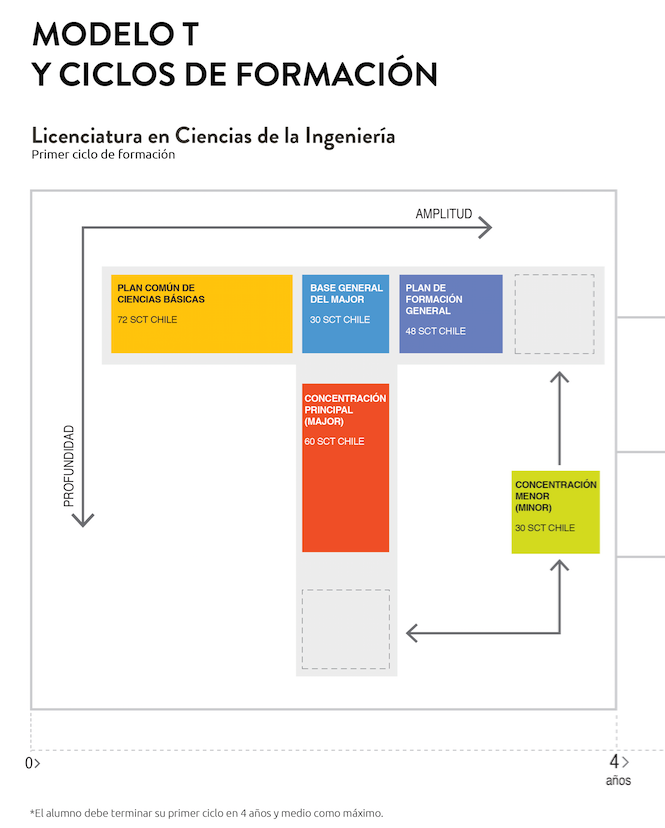
\includegraphics[width=0.5\textwidth]{./figures/model_t.png}
  \setcaptioncitation{\cite{student_manual}}
  \caption{Modelo T en el primer ciclo formativo}
  \label{fig:t_model}
	\end{center}
\end{figure}

De la figura \ref{fig:t_model} cabe destacar que el Minor complementa el aspecto profundidad o amplitud dependiendo del área del Major escogido.

Dado el objetivo de compatibilizar con mallas curriculares internacionales, los ciclos formativos miden su exigencia académica en créditos SCT-Chile, los cuales puede ser transformados a créditos UC gracias a la equivalencia entregada por la universidad. La distribución de carga académica por componente tanto en créditos SCT-Chile como créditos UC se distribuye en la siguiente tabla:

\begin{tabularx}{\linewidth}{@{}c c c@{}}
  \caption{Distribución de créditos SCT-Chile y UC en el primer ciclo formativo} \label{tab:distrution_credits}\\
  \toprule
  Componente & Créditos SCT-Chile & Créditos-UC
  \endhead
  \midrule
  Plan Común de Ciencias Básicas & 72 & 120\\
  \midrule
  Base General del Major & 48 & 80\\
  \midrule
  Plan de Formación General & 48 & 80\\
  \midrule
  Concentración Principal (Major) & 60 & 180\\
  \midrule
  Concentración Menor (Minor) & 30 & 50\\
  \bottomrule
\end{tabularx}

Esta estructura define la malla curricular del primer ciclo formativo, la cual puede ser visualizada en la ilustración \ref{fig:bachelor_study_plan}.

\begin{figure}
	\begin{center}
  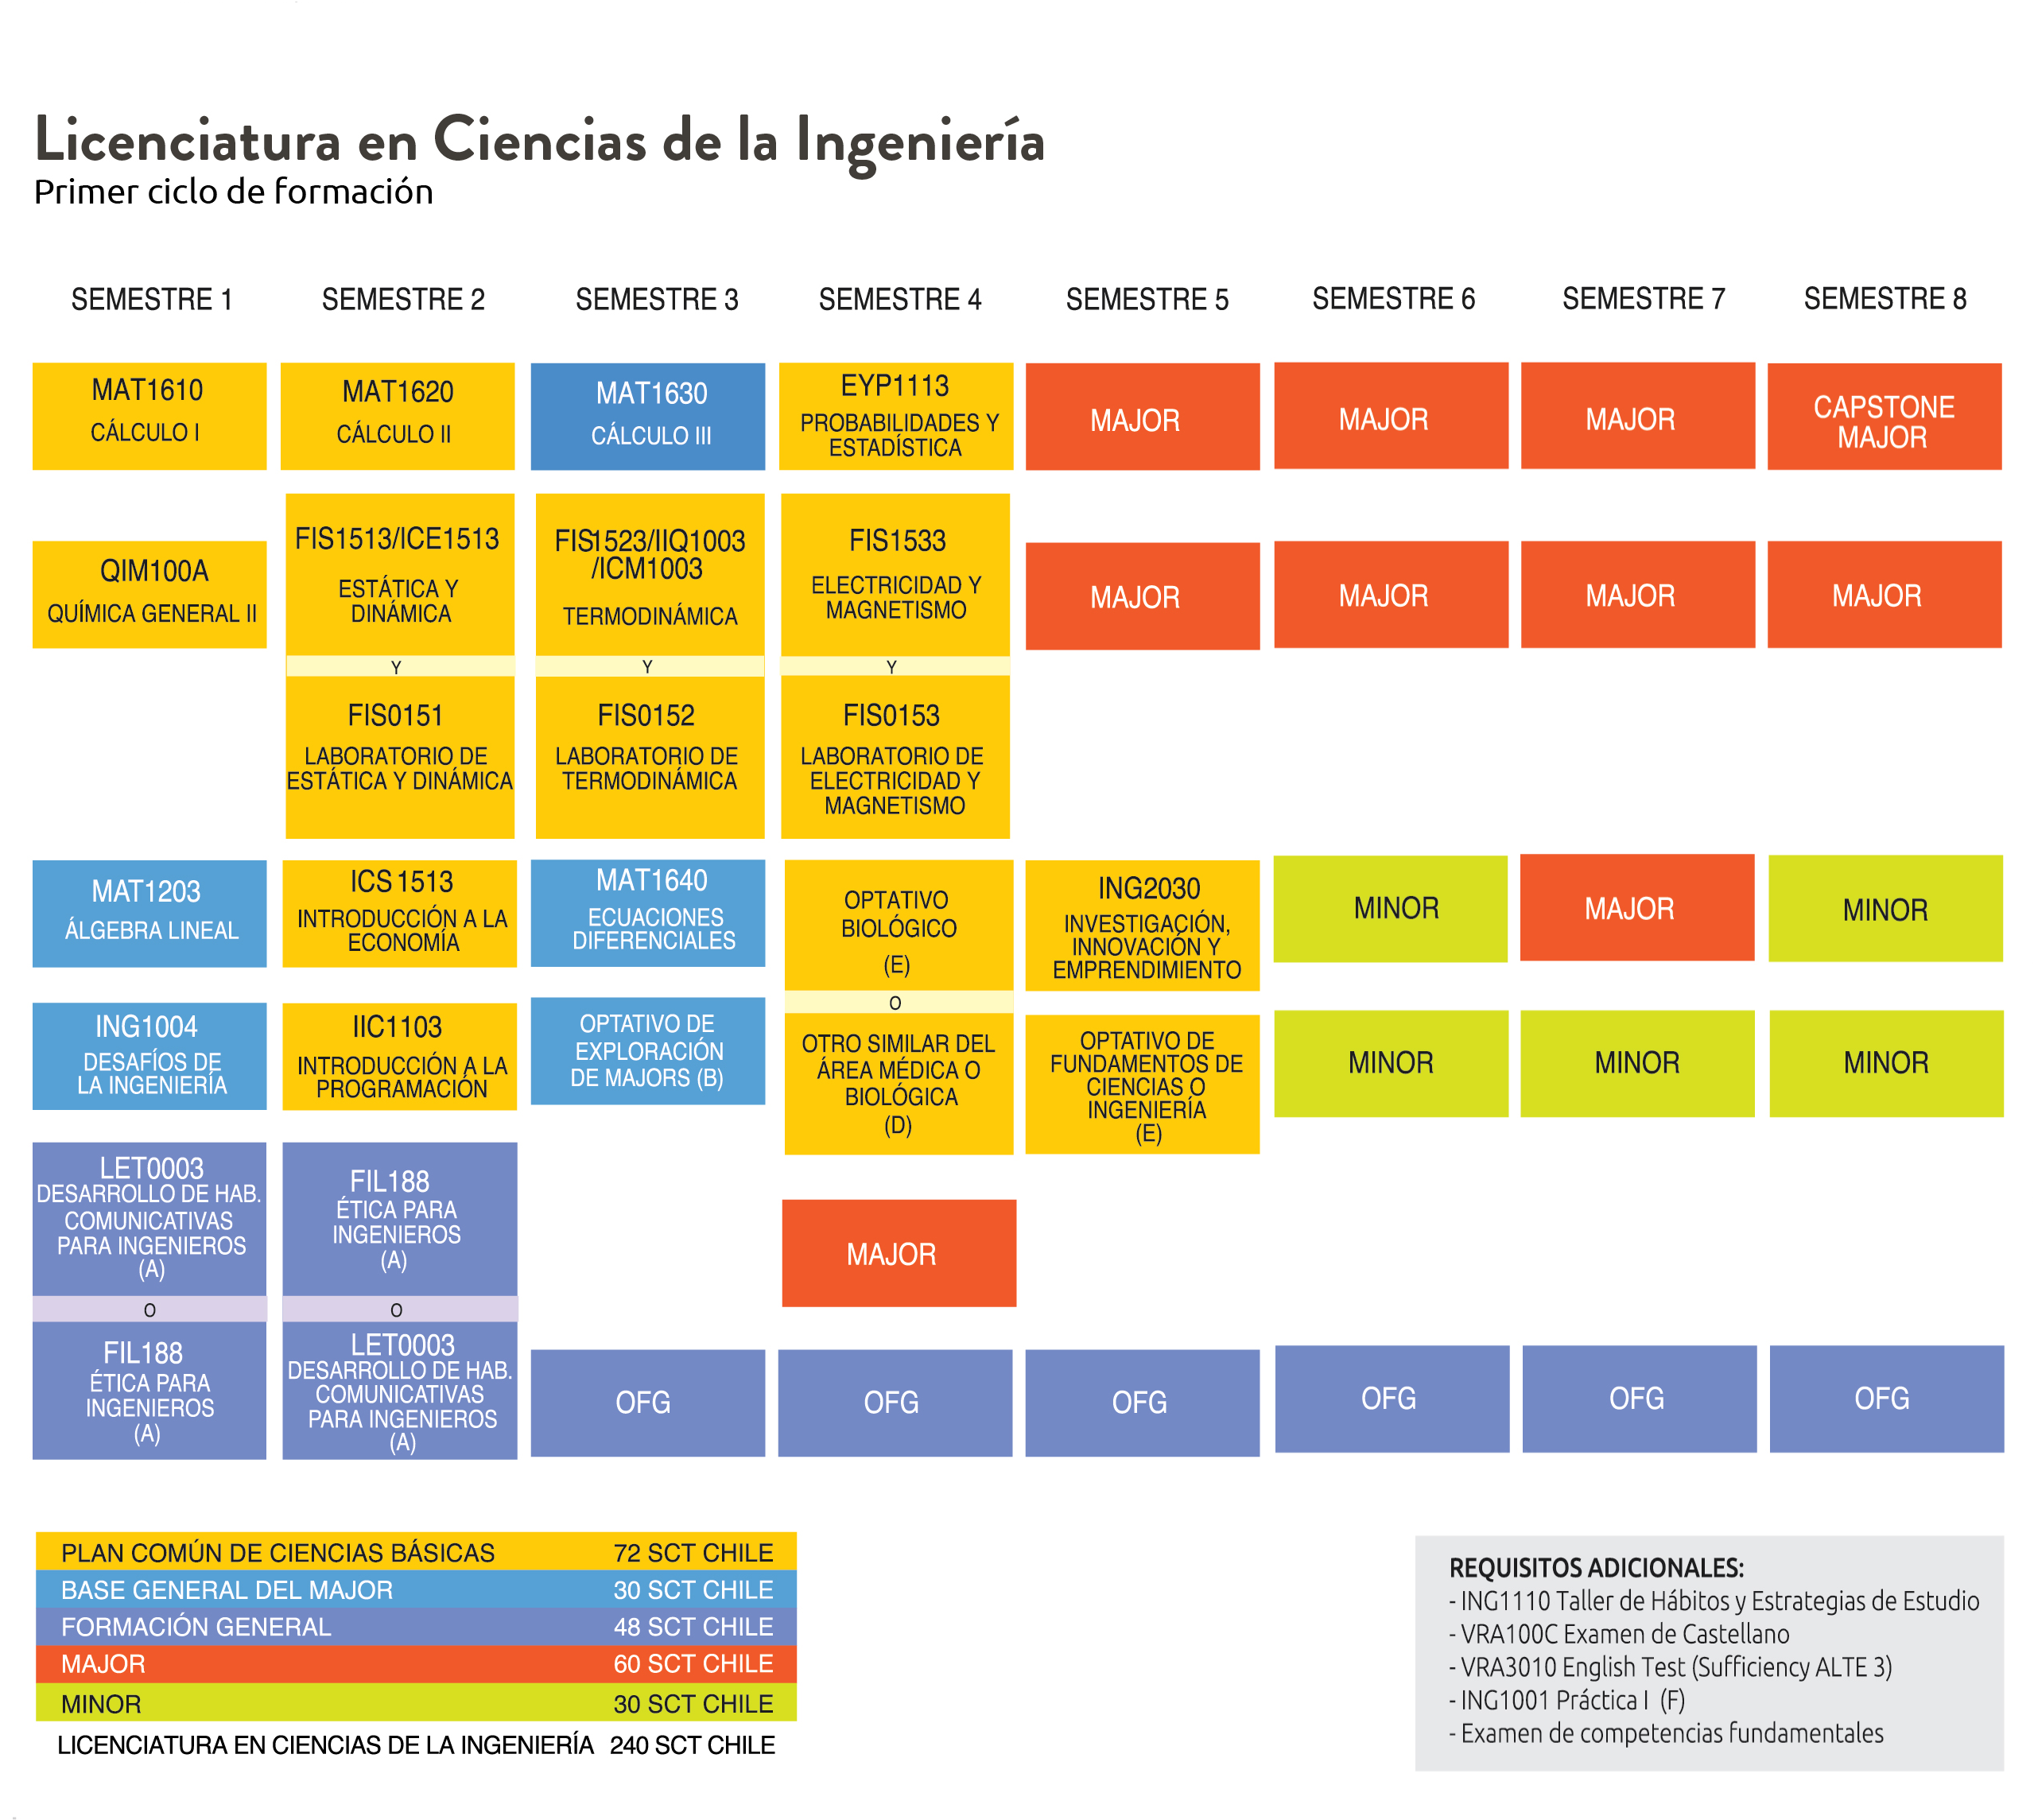
\includegraphics[width=0.7\textwidth]{./figures/malla_curricular.png}
  \setcaptioncitation{\cite{student_manual}}
  \caption{Malla curricular primer ciclo formativo}
  \label{fig:bachelor_study_plan}
	\end{center}
\end{figure}

La diversidad en la formación que puede escoger un alumno se encuentra en la conjunto Major-Minor que escoge, actualmente la Escuela de Ingeniería ofrece un total de 21 Majors, de los cuales 14 son disciplinarios y 7 interdisciplinarios, al mismo tiempo, entrega una oferta de 57 Minors entre los cuales, 32 son profundidad y 25 de amplitud. En el Anexo I se detalla los Majors y Minors disponibles.

Finalmente, con el objetivo de orientar a los alumnos hacia una elección de Major/Minor basada en sus intereses, se les solicita que hagan declaraciones de Major al término del segundo semestre y tercero para terminar con elección de Major y Minor al finalizar su cuarto semestre.

\subsubsection{Continuidad - Articulación Posterior a la Licenciatura \label{sec:degree_structure}}

El segundo ciclo formativo se inicia una vez obtenida la Licenciatura en Ciencias de la Ingeniería, el cual entrega los siguientes caminos a seguir:

\begin{enumerate}
  \item Continuidad a un título profesional de Ingeniería Civil UC.
  \item Continuidad a otros títulos profesionales UC. Hoy existen convenios para continuar estudios a los títulos de Médico Cirujano, Arquitecto y Diseñador UC.
  \item Articulación al título profesional Ingeniería UC y al Magíster en Ciencias de la Ingeniería o el Doctorado en Ciencias de la Ingeniería UC.
  \item Realizar un grado académico superior de postgrado (magister o doctorado) UC u otra.
  \item Salida al Mercado Laboral: Emprendimiento o Empleo Temprano.
\end{enumerate}

\section{Desafíos de información identificados \label{sec:challenges}}

El plan de estudios descrito recientemente fue implementado el año 2013, esto trae consigo una serie de cambios tanto en la comunidad de estudiantes por los nuevos conceptos establecidos como a nivel administrativo para la planificación de cursos para los diferentes ciclos y profesores para los cursos impartidos en cada uno. Esta situación se vuelve particularmente crítica en particular por varios cambios realizados en la planificación inicial de cada Major y/o Minor, así como también en las Articulaciones establecidas entre la Escuela de Ingeniería y otras unidades académicas como Diseño y Medicina. Tanto los cambios como la propia estructura flexible levantan un desafío a nivel de información en cómo realizar un seguimiento adecuado del plan de estudio que realiza cada alumno, para poder disponer de la mejor manera los recursos disponibles por la Escuela.

Las necesidades de información que se detectan para realizar un seguimiento adecuado del plan de estudios de cada alumnos pueden ser descritas en las siguientes categorías:

\begin{enumerate}
  \item Registro de cursos tomados por los alumnos en cada periodo académico.
  \item Registro de las declaraciones de Major realizadas por alumnos por periodo académico.
  \item Gestión de demanda de cursos para cursos, Major y Minor por parte de los alumnos de las diferentes generaciones del nuevo plan.
\end{enumerate}
